\documentclass{article}
\usepackage[utf8]{inputenc}
\usepackage[portuguese]{babel}
\usepackage{listings}
\usepackage{xcolor}
\usepackage{indentfirst}
\usepackage{hyperref}
\setlength{\parindent}{6ex}
\usepackage{graphicx}
\lstset{basicstyle=\ttfamily,
  showstringspaces=false,
  commentstyle=\color{red},
  keywordstyle=\color{blue},
  tabsize=3
}

\title{\textbf{Processamento de Linguagens - TP1a}}
\author{\begin{tabular}{c}
            \textbf{} Carlos Pereira (A61887) \\ João Barreira (A73831) \\ Rafael Costa (A61799)
        \end{tabular}
       }
\date{Março 2017}

\begin{document}

\maketitle

\newpage
\renewcommand*\contentsname{Índice}

\tableofcontents

\newpage
\section{Introdução}

O presente trabalho consiste no desenvolvimento de filtros de texto recorrendo à ferramenta \emph{GAWK}. Os diferentes filtros devem ser produzidos com o recurso a \emph{Expressões Regulares} para detetar \emph{padrões de frases}. Para aumentar estas capacidades, foram propostos quatro exercícios distintos. Neste trabalho, optou-se por resolver todos estes exercícios.

Ao longo deste relatório explicaremos, com detalhe, a resolução de cada exercício proposto. Para cada um é dada ênfase às \emph{Expressões Regulares} e \emph{Ações Semânticas}, bem como eventuais estruturas e variáveis auxiliares utilizadas. Cada secção é também acompanhada pelo código completo do filtro de texto e de um ou mais exemplos da sua execução.

\newpage
\section{Processador de transações da Via Verde}

O ficheiro \emph{viaverde.xml} contém o extrato mensal de um cliente do serviço da Via Verde, fazendo referência à data, aos locais de entrada e saída (e.g. estrada ou parque), ao valor pago e à matrícula do veículo, entre outros.

De acordo com estas informações, foi desenvolvido um processado de texto com o auxílio do \emph{GAWK} para ler o ficheiro \emph{XML} e extrair as meta-informações pedidas.

\subsection{Número total de 'entradas' em cada dia do mês}

Foi feito um processador que lê o ficheiro \emph{XML} e apresenta o número total de entradas para cada um dos dias em cada mês.

\subsubsection{Expressões Regulares e Ações Semânticas}

\begin{itemize}
    \item \textbf{"[\textgreater-]"} - Esta expressão é usada como \textbf{field separator}. Desta maneira, torna-se bastante simples extrair do ficheiro \emph{XML} atributos de cada \emph{tag}, bem como separar os campos de cada uma das datas (mês e dia, nest caso).
    \item \textbf{/\textless data\_entrada\textgreater[0-9]/} - Identifica todas as linhas com informação relativa à data de entrada. Através da utilização do \emph{field separator} em questão, é-nos agora possível aceder ao dia e ao mês das datas de entrada (que estão nos campos 2 e 3, respetivamente).
\end{itemize}

\subsubsection{Estrutura de Dados Globais}

Neste exercício apenas utilizámos um array bidimensional para guardar o mês e o dia de cada uma das entradas registadas no ficheiro \emph{XML}, bem como duas variáveis auxiliares \emph{auxDay} e \emph{auxMonth} que servem apenas para fazer com que o valor retirado dos campos 2 e 3 seja um inteiro (e não uma string).

\subsubsection{Filtro de Texto}

\begin{lstlisting}[language=bash]
BEGIN {
	IGNORECASE = 1;
	FS = "[>-]";
}
/<data_entrada>[0-9]/ {
	auxDay = 0 + $2;
	auxMonth = 0 + $3;
	count[auxMonth][auxDay]++;
}
END {
	for (i = 1; i <= 12; i++) {
		if (i in count) {
			print "Mês: " i;

			for (j = 1; j <= 31; j++) {
				if (j in count[i]) {
					print "\tDia: " j " - " count[i][j] " entradas.";
				}
			} 
		}
	}
}
\end{lstlisting}

\subsubsection{Exemplos de Execução}

\begin{center}
    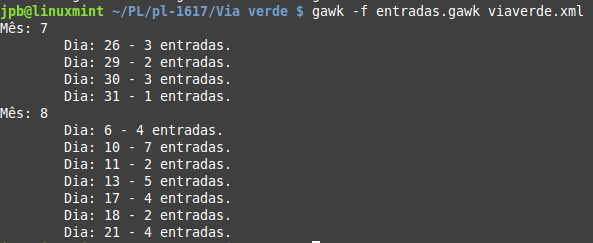
\includegraphics[scale=1]{imagens/entradas}
    \caption{\textbf{Figura 1} - Resultado do filtro de texto \emph{entradas.gawk}}
\end{center}


\subsection{Lista dos locais de 'saída'}

Fez-se um processador que lê o ficheiro \emph{XML} e apresenta a lista dos locais de saída sem repetições e por ordem alfabética.

\subsubsection{Expressões Regulares e Ações Semânticas}

\begin{itemize}
    \item \textbf{"[\textless\textgreater]"} - Esta expressão é usada como \textbf{field separator}. Desta maneira, torna-se bastante simples extrair do ficheiro \emph{XML} atributos de cada \emph{tag}.
    \item \textbf{/\textless saida\textgreater/ && !(\$3 in list)} - Identifica todas as linhas com informação relativa à 'saída' e cujo local de saída (dado pelo campo 3) ainda não esteja no array 'list', que, no fim da execução, conterá o conjunto com os nomes de todos os locais de saída.
\end{itemize}

\subsubsection{Estrutura de Dados Globais}

Para este exercício apenas utilizámos um \emph{array} que contém o nome de todos os locais de saída (ordenado alfabeticamente e sem repetições) presentes no ficheiro \emph{XML}.

\subsubsection{Filtro de Texto}

\begin{lstlisting}
BEGIN {
	IGNORECASE = 1;
	FS = "[><]";
}
/<saida>/ && !($3 in list) {
	list[$3] = $3;
}
END {
	print "Lista de saidas:" 

	for (e in list) {
		print "\t" e;
	}
}
\end{lstlisting}

\subsubsection{Exemplos de Execução}

\begin{center}
    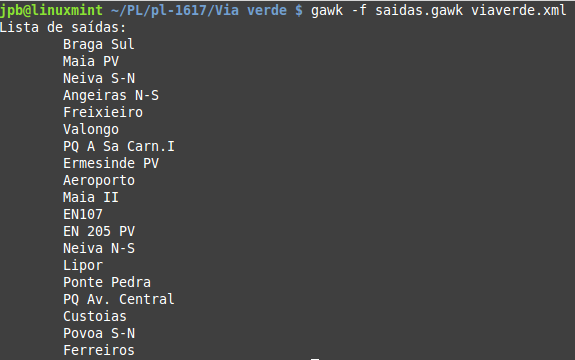
\includegraphics[scale=1]{imagens/saidas}
    \caption{\textbf{Figura 2} - Resultado do filtro de texto \emph{saidas.gawk}}
\end{center}

\subsection{Total gasto no mês (total e apenas em 'parques')}

Para responder às últimas duas alíneas deste exercício, foi desenvolvido um processador que lê o ficheiro \emph{XML} e apresenta os valores mensais do total gasto e o total gasto apenas em parques.

\subsubsection{Expressões Regulares e Ações Semânticas}

\begin{itemize}
    \item \textbf{"[\textless\textgreater]"} - Esta expressão é usada como \textbf{field separator}. Desta maneira, torna-se bastante simples extrair do ficheiro \emph{XML} atributos de cada \emph{tag}.
    \item \textbf{/\textless importancia\textgreater/} - Identifica todas as linhas com informação relativa ao valor pago (i.e. importância).
    \item \textbf{/\textless valor\_desconto\textgreater/} - Identifica todas as linhas com informação relativa ao desconto. O valor final será calculado subtraindo à importância o valor do desconto.
    \item \textbf{/\textless tipo\textgreater parque/} - Identifica todas as linhas com informação relativa ao 'tipo', selecionando apenas aquelas que são do tipo 'parque'.
\end{itemize}

\subsubsection{Estruturas de Dados Globais}

Foram utilizadas as variáveis \emph{imp}, \emph{desc}, \emph{total} e \emph{totalP} para guardar, respetivamente, a importância, o desconto, o gasto total e o gasto em 'parques'.

\subsubsection{Filtro de Texto}

\begin{lstlisting}
BEGIN {
	IGNORECASE = 1;
	FS = "[><]";
}
/<importancia>/ {
	sub(",", ".", $3);
	imp = $3;
}
/<valor_desconto>/ {
	sub(",", ".", $3);
	desc = $3;
	total += imp - desc;
}
/<tipo>parque/ {
	totalP += imp - desc;
}
END {
	print "Total gasto: " total;
	print "Total gasto em parques: " totalP;
}
\end{lstlisting}

\paragraph{}
\subsubsection{Exemplos de Execução}

\begin{center}
    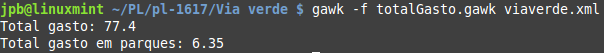
\includegraphics[scale=1]{imagens/totalGasto}
    \caption{\textbf{Figura 3} - Resultado do filtro de texto \emph{totalGasto.gawk}}
\end{center}

\newpage
\section{Album fotográfico em HTML}

O principal objetivo deste exercício consiste em extrair toda a meta-informação de um ficheiro, em formato \emph{XML}, e gerar uma página \emph{HTML} com essa meta-informação. Esse ficheiro, chamado \emph{lengenda.xml}, possui informação acerca de um conjunto de ficheiros de fotografias e, para cada uma destas, o nome das pessoas envolvidas e o local onde foram tiradas. A página \emph{HTML} deve apresentar todas a fotos listadas no ficheiro \emph{XML}, bem como as pessoas envolvidas em cada uma. Para além disso, deve ser gerada a lista de todos os locais envolvidos, sem repetições. De referir que os ficheiros das fotografias encontram-se em \url{http://npmp.epl.di.uminho.pt/images/}.

Optou-se por gerar a página \emph{HTML} de duas maneiras distintas: através do comando \emph{IMG} e através de uma âncora com o hiper-link que associe o nome do fotografado ao ficheiro. Apresentam-se, nas secções seguintes, os detalhes de cada uma destas implementações.


\subsection{Página \emph{HTML} com comandos \emph{IMG}}

Esta implementação gera uma página \emph{HTML} com o seguinte formato:

\begin{lstlisting}[language=html]
    <LI><b>NomeDaPessoa</b></LI>
        <center><img src="NomeDoFicheiro.jpg"/></center>
\end{lstlisting}


\subsubsection{Expressões Regulares e Ações Semânticas}

\begin{itemize}
    \item \textbf{"[\textless\textgreater/"]"} - Esta expressão é usada como \emph{FIELD SEPARATOR}. Desta maneira, torna-se bastante simples extrair do ficheiro \emph{XML} atributos de cada \emph{tag}, bem como nomes de ficheiros entre aspas. 
    \item \textbf{/\textless foto / } - Identifica todas as linhas com informação relativa a uma foto. Como se pode verificar, na definição do \emph{FIELD SEPARATOR}, o nome do ficheiro de uma foto é armazenado no campo número três. Basta armazenar-se o valor desse campo numa variável auxiliar.
    \item \textbf{/\textless quem\textgreater/} - A identificação dos sujeitos envolvidos numa foto é armazenada no campo número três. Usa-se uma função auxiliar para limpar todos os espaços em branco tanto no início como fim da descrição. No final, é acrescentada a informação de uma imagem em formato \emph{HTML} a um ficheiro chamado \emph{index.html}.
    \item \textbf{/\textless onde\textgreater/ && !((\$3 = removeSpaces(\$3)) in locals)} - Filtra todas as linhas que possuam informações do local onde foi tirada uma foto. Uma linha é selecionada se contiver informação de um local que ainda não tenha sido armazenado. Caso estas condições se verifiquem, o local (presente no campo número três) é guardado num \emph{array}. 
\end{itemize}


\subsubsection{Estruturas de Dados Globais}

As estruturas globais envolvidas neste exercício são as seguintes: um \emph{array locals} para guardar todos os locais (sem repetições) onde foram tiradas as fotos e quatro variáveis globais. Três das variáveis (\emph{fmtLI}, \emph{fmtI} e \emph{end}) possuem valores constantes relativos a código \emph{HTML}. A quarta variável (\emph{image}) serve para guardar o ficheiro da última foto lida.


\subsubsection{Filtro de Texto}

\begin{lstlisting}[language=bash]
BEGIN {
	IGNORECASE = 1;
	fmtLI = "<li><b>%s</b></li>\n";
	fmtI = "<center><img src=
	        \"http://npmp.epl.di.uminho.pt/images/%s\"/> 
	        </center>\n"
	FS = "[<>\"]";
	end = "</body></html>";
	print "<html><head><meta charset='UTF-8'/>
	       </head><body>" > "index.html";
}

/<foto / {
	file = $3;
}

/<quem>/ {
	$3 = removeSpaces($3);

	printf(fmtLI, $3) > "index.html";
	printf(fmtI, file) > "index.html";
}

/<onde>/ && !(($3 = removeSpaces($3)) in locals) {
	locals[$3] = 0;
}

END {
	print "<p></p>\n<b>Locais:</b>\n" > "index.html";
	
	for (i in locals) {
		printf("<li>%s</li>\n", i) > "index.html";
	}

	print end > "index.html";
}

function removeSpaces(str) {
	sub("^ +", "", str);
	sub(" +$", "", str);

	return str;
}

\end{lstlisting}

\subsubsection{Exemplos de Execução}

Apresentam-se de seguida, parte do ficheiro \emph{legenda.xml} (\textbf{Figura 4}) e o respetivo resultado numa página \emph{HTML} (\textbf{Figura 5}).

\begin{center}
    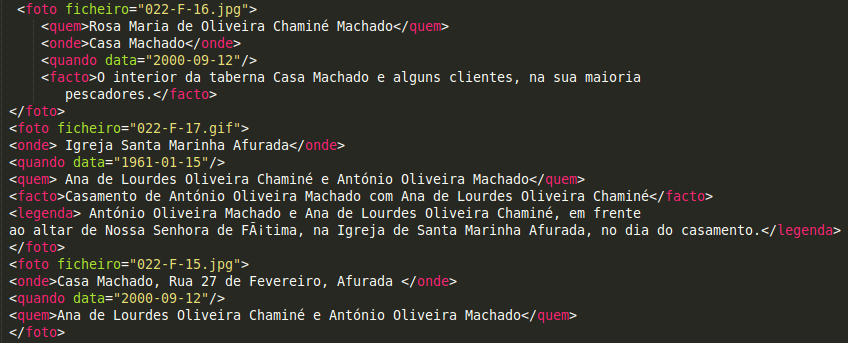
\includegraphics[scale=0.7]{imagens/legenda}
    \caption{\textbf{Figura 4} - Parte do ficheiro \emph{legenda.xml} com três fotos distintas}
\end{center}

\begin{center}
    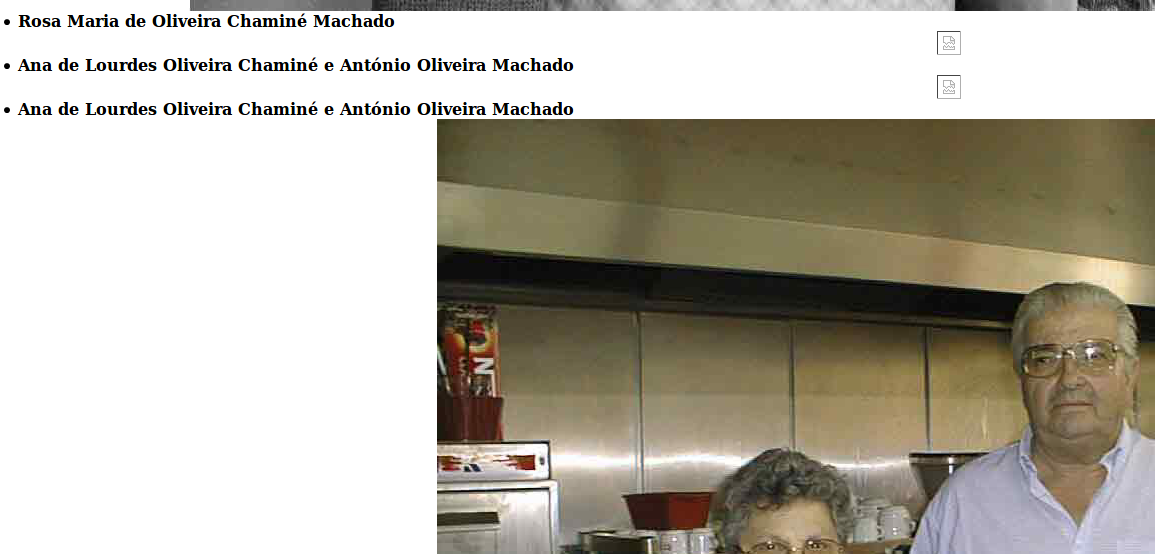
\includegraphics[scale=0.51]{imagens/foto}
    \caption{\textbf{Figura 5} - Porção da página \emph{HTML} resultante}
\end{center}

\newpage
Todos os diferentes locais são listados no final da página \emph{HTML} de acordo com a seguinte figura:

\begin{center}
    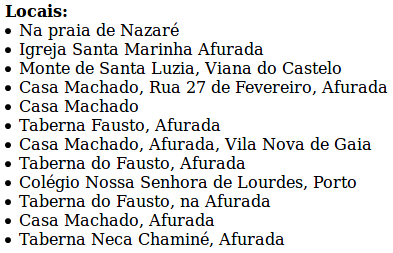
\includegraphics[scale=1]{imagens/locais}
    \newline\caption{\textbf{Figura 6} - Lista de todos os locais onde foram tiradas as fotos}
\end{center}

\subsection{Página \emph{HTML} com âncoras}
Esta implementação é muito semelhante à implementação com o comando \emph{IMG} mas, acrescenta uma nova funcionalidade. O conjunto de pessoas envolvidas no album é apresentado sem repetições. Cada pessoa tem a si associada uma página \emph{HTML} que dispõe todos as fotos em que está presente. De seguida faremos referência apenas às expressões regulares e ações semânticas que divirgem da implementação com \emph{IMG}.


\subsubsection{Expressões Regulares e Ações Semânticas}
A única expressão regular que é distinta das expressões regulares da outra implementação é a seguinte: \textbf{/\textless quem\textgreater/ && (length(\$3) \textless 200)}. Esta expressão filtra todas as linhas com a \emph{tag quem} em que o nome da pessoa envolvida não ultrapasse os duzentos carateres (de modo a evitar erros ao guardar ficheiros com um nome demasiado extenso).  



\subsubsection{Estruturas de Dados Globais}
Tal como na implementação com \emph{IMG} são utilizadas um conjunto de variáveis constantes que contêm código \emph{HTML}, uma variável para guardar o nome do ficheiro de uma foto e um \emph{array} de locais. Para além destas estruturas é utilizado um \emph{array} de duas dimensões \emph{album[quem][images]}, que associa a uma pessoa um conjunto de fotos onde está presente.

\newpage

\subsection{Filtro de Texto}
\begin{lstlisting}[language=bash]
BEGIN {
	IGNORECASE = 1;
	enc = "<html> <head> <meta charset='UTF-8'/>
	       </head> <body>"
	fmtHREF = "<p><a href=\"%s.html\"> %s </a></p>\n";
	fmtIMG = "<li><center><img 
	          src=\"http://npmp.epl.di.uminho.pt/images/%s\"/> 
	          </center></li>\n"
	FS = "[<>\"]";
	end = "</body></html>";
	print enc > "index.html";
}


/<foto / {
	image = $3;
}

/<quem>/ && (length($3) < 200) {
	$3 = removeSpaces($3);
	array[$3][image] = 0;
}

/<onde>/ && !(($3 = removeSpaces($3)) in locals) {
	locals[$3] = 0;
}

END {
	for (i in array) {
		aux = removeInvalidChars(i);

		printf(fmtHREF, aux, i) > "index.html";

		print enc > aux".html";

		for (j in array[i]) {
			printf(fmtIMG, j) > aux".html";
		}

		print end > aux".html";
	}

	print "<p></p>\n<b>Locais:</b>\n" > "index.html";
	
	for (x in locals) {
		printf("<li>%s</li>\n", x) > "index.html";
	}

	print end > "index.html";
}

function removeSpaces(str) {
	sub("^ +", "", str);
	sub(" +$", "", str);

	return str;
}


function removeInvalidChars(str) {
	sub("[:\\t]", "", str);
	return str;
}

\end{lstlisting}

\subsubsection{Exemplos de Execução}

Aproveitemos o exemplo fornecido no exercício anterior (\textbf{Figura 4}). O resultado é o seguinte:

\begin{center}
    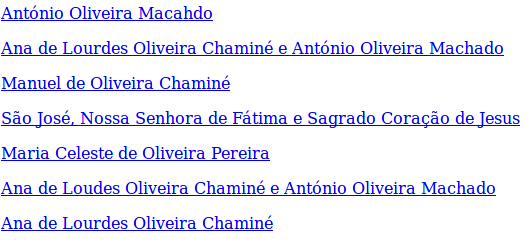
\includegraphics[scale=1]{imagens/pessoas}
    \newline\caption{\textbf{Figura 7} - Porção da página \emph{HTML} resultante}
\end{center}

A listagem com os locais onde foram tiradas as fotos aparece no fundo da página \emph{HTML}, como no exercício anterior (\textbf{Figura 6}).

\newpage
\section{Autores musicais}

Existe uma diretoria com vários ficheiros de extensão '\emph{.lyr}', que contêm a letra de canções precedida de dois ou mais campos de meta-informação (um por linha). Esta informação pode ser: título da canção, autor da letra, cantor, etc. A letra da música e a meta-informação estão separadas por uma linha em branco.

Foi feito um Processador de Texto com o auxílio do \emph{GAWK} para ler todos os ficheiros '\emph{.lyr}' e obter informações sobre os cantores, autores e títulos de canções.

\subsection{Total de \emph{cantores} e a lista com os nomes}

Aqui foi feito um processador que recebe ficheiros de letra de música como \emph{input} e escreve o total e os nomes de todos os cantores.

\subsubsection{Expressões Regulares e ações semânticas}


\begin{itemize}
    \item \textbf{" *[:;,]"} - Esta expressão é usada como \emph{FIELD SEPARATOR}.
    \item \textbf{/\textless singer:/ } - Identifica todas as linhas com informação relativa a um cantor. Na definição do \emph{FIELD SEPARATOR}, os nomes dos cantores de uma música começam a partir do campo número dois. Após feita a remoção de carateres desnecessários, os valores desses campos são guardados num \emph{array} em que o índice é o nome do cantor. O contador do número de cantores é incrementado.
\end{itemize}

No fim imprimem-se os nomes de todos os cantores e o total.

\subsubsection{Estruturas de Dados Globais}

Foram utilizadas duas estruturas de dados globais: um \emph{array} \emph{singers}, em que o índice são os nomes de todos os cantores e uma variável \emph{total} que é utilizada como contador de cantores.

\subsubsection{Filtro de Texto}

\begin{lstlisting}[language=bash]
BEGIN {
	FS = " *[:;,] *"
}

/singer:/ {
	for (i = 2; i <= NF; i++) {
	    sub("[ ?()]+$", "", $i);

	    if (!($i in singers) && ($i != "")) {
	    	count++;
	    	singers[$i] = $i;
	    }
	}
}

END {
	n = asort(singers);

	for (i = 1; i <= n; i++) {
		print singers[i];
	}

	print "Total: " count;
}
\end{lstlisting}

\subsubsection{Exemplos de Execução}

\begin{center}
    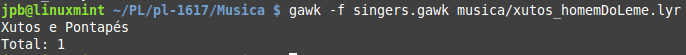
\includegraphics[scale=1]{imagens/singers_1}
    \caption{\textbf{Figura 8} - Resultado da execução do filtro de texto aplicado ao ficheiro \emph{xutos\_homemDoLeme.lyr}}
\end{center}

\paragraph{}

\begin{center}
    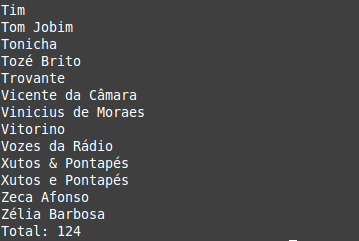
\includegraphics[scale=1]{imagens/singers_all}
\end{center}   
\begin{center}
    \caption{\textbf{Figura 9} - Parte do resultado do filtro de texto aplicado a todos os ficheiro '\emph{.lyr}'
\end{center}

\subsection{Todas as canções do mesmo \emph{autor}}

Fez-se um processador que recebe ficheiros de letra de música como \emph{input} e calcula o número de canções de cada autor.

\subsubsection{Expressões Regulares e Ações Semânticas}

\begin{itemize}
    \item \textbf{" *[:;,]"} - Esta expressão é usada como \emph{FIELD SEPARATOR}.
    \item \textbf{/\textless author:/ } - Identifica todas as linhas com informação relativa a um autor. Na definição do \emph{FIELD SEPARATOR}, os nomes dos autores de uma música começam a partir do campo número dois. Após feita a remoção de carateres desnecessários, os valores desses campos são guardados num \emph{array} em que o índice é o nome do cantor e o valor correspondente a esse índice é o número de músicas desse autor. Este contador também é incrementado.
\end{itemize}

No fim, imprimem-se os resultados da seguinte forma: nome do autor seguido do número de músicas associadas a ele.

\subsubsection{Estruturas de Dados Globais}

Temos como estrutura global um \emph{array} \emph{authors}, em que o índice é o nome de um autor e o valor correspondente ao número de músicas associado a esse autor. 

\subsubsection{Filtro de Texto}

\begin{lstlisting}[language=bash]

BEGIN {
	FS = " *[:;,] *"
}

/author:/ {
	for (i = 2; i <= NF; i++) {
		sub("[ ?()\\t]+$", "", $i);

		if ($i != "") {
			songs[$i]++;
		}
		else {
			songs["Autor desconhecido"]++;
		}

	}
}

END {
	for (i in songs) {
		print i " - " songs[i];
	}
}

\end{lstlisting}

\subsubsection{Exemplos de Execução}

\begin{center}
    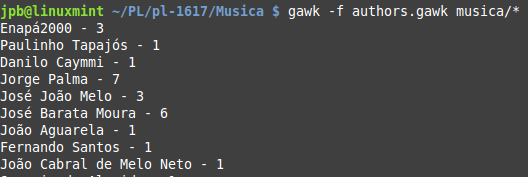
\includegraphics[scale=1]{imagens/authors}
    \caption{\textbf{Figura 10} - Resultado da execução do filtro de texto \emph{authors.gawk}
\end{center}

\subsection{Escrever o nome de cada \emph{autor} seguido do título das suas canções}

\paragraph{} O processador recebe ficheiros de letra de música como \emph{input} e escreve, para cada autor, o título das suas canções.

\subsubsection{Expressões Regulares e Ações Semânticas}


\begin{itemize}
    \item \textbf{" *[:;,]"} - Esta expressão é usada como \emph{FIELD SEPARATOR}.
    \item \textbf{/title :/} - As informações relativas aos títulos das canções começam por esta expressão. Quando isto se verificar, o título é guardado numa variável global.
    \item \textbf{/author:} - Os autores de uma canção aparecem depois desta expressão, a partir do campo número dois. Após a remoção de carateres desnecessários, o título da canção é adicionado a uma matriz cujo índice de linha é o nome do autor e o índice de coluna o título da canção.
    
    Caso não se saiba quem são os autores, o título da canção é adicionado ao \emph{Autor Desconhecido}.
    
\end{itemize}

No fim, para cada uma das linhas da matriz \emph{songs}, imprime-se para cada linha, o seu índice e os conteúdos de cada uma das suas colunas.

\subsubsection{Estruturas de Dados Globais}

Utilizaram-se duas variáveis globais: a variável \emph{song} que guarda o título de uma canção e uma matriz \emph{songs}. Nesta matriz, as linhas correspondem a nome de autores e as respetivas colunas correspondem aos títulos das canções associadas ao autor dessa linha.

\newpage
\subsubsection{Filtro de Texto}

\begin{lstlisting}[language=bash]
BEGIN {
	FS = " *[:;,] *"
}

/title: / {
	song = $2;
	sub("\\(\\?\\)", "", song);
	sub("^[ *=]+", "", song);
}

/author:/ {
	for (i = 2; i <= NF; i++) {
		sub("[ ?()\\t]+$", "", $i);

		if ($i != "") {
			authors[$i][song] = song;
		}
		else {
			authors["Autor desconhecido"][song] = song;
		}

	}
}

END {
	for (a in authors) {
		printf("%s: ", a);

		flag = 0;		

		for (j in authors[a]) {
			if (flag == 0) {
				printf("%s", j);
			}
			else {
				printf(", %s", j);
			} 

			flag++;
		}

		printf("\n");
	}
}
\end{lstlisting}

\subsubsection{Exemplos de Execução}

\begin{center}
    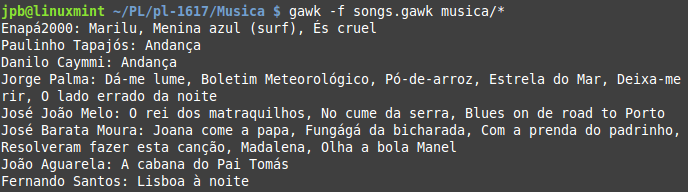
\includegraphics[scale=1]{imagens/songs}
    \caption{\textbf{Figura 11} - Resultado da execução do filtro de texto \emph{songs.gawk}}
\end{center}


\newpage
\section{Dicionauro}

Uma diretoria designada por \emph{Dicionauro} contém um conjunto de ficheiros com a extensão '\emph{.txt}' com inúmeras entradas em Português de termos de um \emph{Thesaurus}. Cada termo é iniciado pela sigla '\emph{PT}' e tem a si associado uma ou mais categorias. Um termo pode possuir um conjunto de definições. Uma definição é uma linha iniciada pela sigla '\emph{Def}'. 

Descrevem-se, de seguida, os exercícios propostos que têm como base a diretoria \emph{Dicionauro}.  


\subsection{Criação de uma página \emph{HTML} com todos os termos e suas respetivas categorias e definições}

A estrutura da página \emph{HTML} criada neste exercício é a seguinte:

\begin{lstlisting}[language=html]
<p></p><b>Termo</b>
<p></p><b>Categorias:</b>
<li>Categoria 1</li>
<li>Categoria 2</li>
          .
          .
          .
        
<p></p><b>Definicoes:</b>
<li>Definicao 1</li>
<li>Definicao 2</li>
          .
          .
          .
\end{lstlisting}


Ou seja, na leitura de todos os ficheiros presentes na diretoria \emph{Dicionauro} não se devem apresentar termos repetidos, mas sim acrescentar a um termo que já exista novas categorias e definições.


\subsubsection{Expressões Regulares e Ações Semânticas}

\begin{itemize}
    \item \textbf{"[ \textgreater!\textless]*pt(\_br)?(\_pt)?"} - Expressão regular atribuída ao \emph{FIELD SEPARATOR}. Ao inspecionarmos vários ficheiros da diretoria em questão, verificamos que nem todos seguem o mesmo padrão. A maior parte dos ficheiros apresenta as linhas respetivas a um termo iniciadas pela sigla '\emph{PT}'. No entanto, verificamos que um pequeno número de ficheiros possuía a sigla '\emph{PT}' precedida ou sucedida pelo seguinte conjunto de carateres: \emph{\textless, \textgreater, ! e espaço}. Para além disso, uma pequena minoria apresentava distinções para termos em português e em brasileiro, ou seja, '\emph{PT\_PT}' e '\emph{PT\_BR}'. A expressão regular descrita permite tratar cada um destes diferentes tipos de termos. 
    \item \textbf{/\^{}pt/\hspace{0.5em}\textbar\textbar\hspace{0.5em}/\^{}[\textgreater\textless! ]*pt/} - Filtra todos as linhas correspondentes a um termo. Tal como foi, falado acima, existem vários formatos para uma linha com um termo. Todos os espaços em branco (tanto no início como no final) de um termo são extraídos, bem como todos os \emph{tabs} que possua. Depois dessa extração, o termo é guardado numa variável auxiliar.
    \item \textbf{/[ \textless\textgreater!?]*def/} - Esta expressão permite selecionar todas as linhas que contenham uma definição. Novamente a sintaxe de uma linha que contém uma definição pode ser constituída por um conjunto diferente de carateres. Como o \emph{FIELD SEPARATOR} foi definido de modo a selecionar todos os termos de um ficheiro, é necessário recorrer-se ao uso da função \emph{split} para se extrair a definição propriamente dita. Basta usar-se esta função para o campo número zero (todo o registo) e fazer-se o \emph{split} pela sequência de carateres "\emph{def}". 
    \item \textbf{/[ \textless\textgreater!?-]*catgra/} - Seleciona todas as linhas que contêm uma categoria. Tal como para uma definição, é realizado um \emph{split} no campo número zero, mas desta vez pela sequência de carateres "\emph{catgra}".
\end{itemize}


\subsubsection{Estruturas de Dados Globais}

Este exercício recorre ao uso de cinco variáveis auxiliares, de valor constante, para armazenarem meramente código \emph{HTML}. São utilizadas mais três variáveis (\emph{entry}, \emph{def} e \emph{catg}) para guardarem, respetivamente, os valores de um termo, definição e uma categoria. A estrutura mais relevante para este exercício consiste num \emph{array} de três dimensões \emph{entries[entry][catg][def]}. Cada termo deste \emph{array} tem a si associado um conjunto de categorias. Por sua vez, cada categoria tem a si associada um conjunto de definições. Esta estruturação é útil em casos em que uma nova categoria é definida para um mesmo termo noutro ficheiro. De modo a facilitar a compreensão desta estrutura ilustraremos o seguinte exemplo: suponha-se que existem três ficheiros distintos ("A", "B" e "C"). Ambos os ficheiros possuem o mesmo termo ("\emph{corpo}") e um conjunto de definições distintas para este. Suponha-se, também, que no ficheiro "A" a categoria do termo é "\emph{nl}" (tal como no ficheiro "B") e que no ficheiro "C" não há nenhuma informação relativa à categoria do termo. Sendo assim o \emph{array} possui as seguintes configurações: \emph{entries["corpo"]["nl"]["conjunto de definições do ficheiro "A" e "B""]} e \emph{entries["corpo"][\" "]["conjunto de definições do ficheiro "C"]}.


\subsubsection{Filtro de Texto}

\begin{lstlisting}[language=bash]
BEGIN {
	IGNORECASE = 1;
	fmtLI = "<li styl, =\"margin-left:50px\">%s</li>\n";
	fmtE = "<p></p><b style=\"font-size:150%\">%s</b>\n"; 
	fmtCD = "<p></p><b style=\"margin-left:25px\">%s</b>\n";
	FS = "^[> !<]*pt(_br)?(_pt)?";
	end = "</body></html>";
	print "<html><head><meta charset='UTF-8'/>
	       </head><body>" > "index.html";
}


/^pt/ || /^[>< !]*pt/ {
	entry = removeWhiteSpaces($2);
}

/[> <!?]*def/ {
	split($0, target, "def");
	def = removeWhiteSpaces(target[2]);
	entries[entry][catg][def] = def;
}

/[> <!?-]*catgra/ {
	split($0, target, "catgra");
	catg = removeWhiteSpaces(target[2]);
}

END {
	for (i in entries) {
		if (length(i) > 1) {
		printf(fmtE, i) > "index.html";
		
		printf(fmtCD, "Categorias:") > "index.html";
		
		for (c in entries[i]) {
			if (length(c) > 1) {
				printf(fmtLI, c) > "index.html";
			}
		}

		printf(fmtCD, "Definições:") > "index.html";

		for (j in entries[i]) {
			for (w in entries[i][j]) {
					if (length(w) > 1) {
						printf(fmtLI, w) > "index.html";
					}
				} 
			}
		}
	}

	print end > "index.html";
}

function removeWhiteSpaces(str) {
	sub("\\t", "", str);
	sub("^ +", "", str);
	sub(" +$", "", str);

	return str;
}

\end{lstlisting}

\subsubsection{Exemplos de Execução}

Como o termo '\emph{costas}' aparece em vários ficheiros, aparecem também várias entradas no ficheiro \emph{HTML} resultante (\textbf{Figura 12}).

\begin{center}
    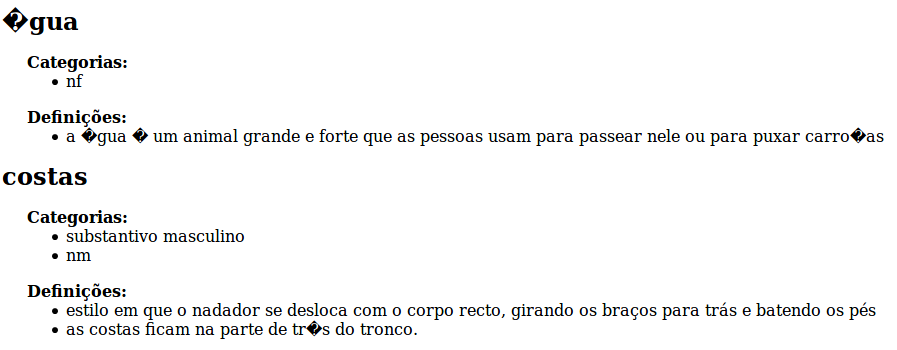
\includegraphics[scale=0.7]{imagens/entradas_all}
    \caption{\textbf{Figura 12} - Resultado da execução do filtro de texto '\emph{entradas.gawk}'}
\end{center}

\subsection{Listagem de todos os diferentes domínios e respetivo número de entradas}

A última alínea deste exercício corresponde a uma listagem de todos os domínios distintos presentes nos ficheiros da diretoria \emph{Dicionauro}. Para além disso, deve-se indicar para cada domínio a quantidade de termos pertencentes.


\subsubsection{Expressões Regulares e Ações Semânticas}

\begin{itemize}
    \item \textbf{"\^{}[& \textgreater!\textless]*dom +"} - Expressão atribuída ao \emph{FIELD SEPARATOR}. Verificou-se que, em certos ficheiros, uma linha que caracteriza um domínio é iniciada pelo seguinte conjunto de carateres: \emph{espaço, &, \textgreater, ! e \textless}. Para além disso, em algumas linhas a palavra \emph{dom} é sucedida por um ou mais espaços.
    \item \textbf{/\^{}[ &\textgreater\textless!]*dom / && length(\$2) \textgreater 0} - Filtra todas as linhas que contenham informação acerca de um domínio não vazio. O domínio é guardado num \emph{array} e, caso este já exista, incrementado o seu número de termos.  
\end{itemize}


\subsubsection{Estruturas de Dados Globais}

Nesta alínea apenas foi usada a seguinte estrutura de dados: um \emph{array} chamado \emph{dom} em que os seus 
índices correspondem a diferentes domínios. Em cada posição do \emph{array dom} consta o número de termos correspondentes.

\subsubsection{Filtro de Texto}

\begin{lstlisting}[language=bash]
BEGIN {
	IGNORECASE = 1;
	FS = "^[&> !<]*dom +";
}

/^[&>< !]*dom / && length($2) > 0 {
	dom[norm($2)]++;
}

END {
	for (i in dom) {
		print i ": " dom[i];
	}
}

function norm(str) {
	sub("^ +", "", str);
	sub(" +$", "", str);
	return tolower(str);
}

\end{lstlisting}

\newpage
\subsubsection{Exemplos de Execução}


\begin{center}
    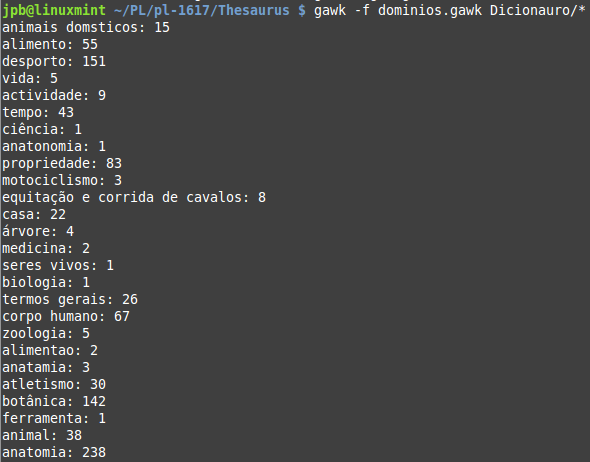
\includegraphics[scale=0.7]{imagens/dominios}
    \newline\caption{\textbf{Figura 13} - Resultado da execução do filtro de texto '\emph{dominios.gawk}'}
\end{center}

\newpage
\section{Conclusão}

Com a realização deste trabalho, pudemos pôr em prática os conceitos adquiridos nas aulas teórico-práticas sobre a ferramenta \emph{GAWK}.

Percebemos a importância do uso das expressões regulares e ações semânticas, de forma a podermos pegar num ficheiro, obter as informações que necessitamos e, com elas, chegar a um conjunto de conclusões.

Tomámos consciência de que esta tarefa nem sempre é fácil (devido à complexidade dos textos em questão), o que faz com que a definição das expressões regulares para conseguirmos obter as informações que necessitamos nem sempre seja uma tarefa trivial. Um bom exemplo deste tipo de dificuldade, foi a nossa tentativa de separar as pessoas no ficheiro \emph{xml} do exercício 2 relativo ao álbum de fotografias.

Assim sendo, em retrospetiva, achamos que a realização deste primeiro trabalho prático foi enriquecedora e nos deu uma boa base relativamente ao processamento de ficheiros textuais.

\end{document}
